\section{From a useful signal to an exposure decision}\label{sec:1}

Suppose AMD and NVDA face similar news, but AMD options become unusually expensive relative to NVDA options. Selling the richer options and buying the cheaper ones expresses a view about the relative price of volatility. Daily stock hedges reduce immediate directional exposure, and initial vega matching reduces sensitivity to a common small change in implied volatility. The trade still carries risk: related stocks can experience different events, and option premiums may correctly reflect those differences.


Our starting point is Ning and Lee's equity-pairs framework \cite{ning2024}, which separates constructing a spread from learning how to trade it. We carry that distinction into options. First, we ask whether an economic rule produces useful historical trades under explicit contract and funding assumptions. We then ask whether learning improves the amount of capital assigned to those opportunities. A profitable signal and a useful allocation policy are separate findings.


\begin{figure}[!htbp]\centering
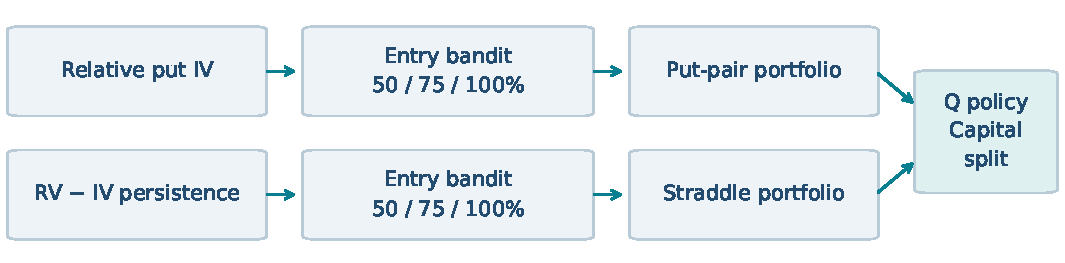
\includegraphics[width=\linewidth]{learning_pipeline.pdf}
\caption{Two exposure decisions. Entry policies size proposals within each signal; a separately fitted Q policy chooses the capital split between funded strategy indices.}\label{fig:learning-pipeline}
\end{figure}

The original relative-volatility strategy remains the foundation of this paper. We add a second signal---persistent realized-minus-implied volatility---and a second learning decision: allocating capital between the resulting strategies. Entry bandits choose individual trade sizes; fitted Q-learning chooses the strategy mix. Both reporting periods, 2018--2021 validation and January 2022--August 2025 evaluation, remain visible throughout.
